\begin{frame}
\frametitle{WP Apprentissage} 
\begin{minipage}{6cm}
L'objectif de ce groupe de travail est à partir de nombreux exercices, de créer des tactiques spécifiques à ce type d'exercice.
\end{minipage}
\begin{minipage}{4cm}
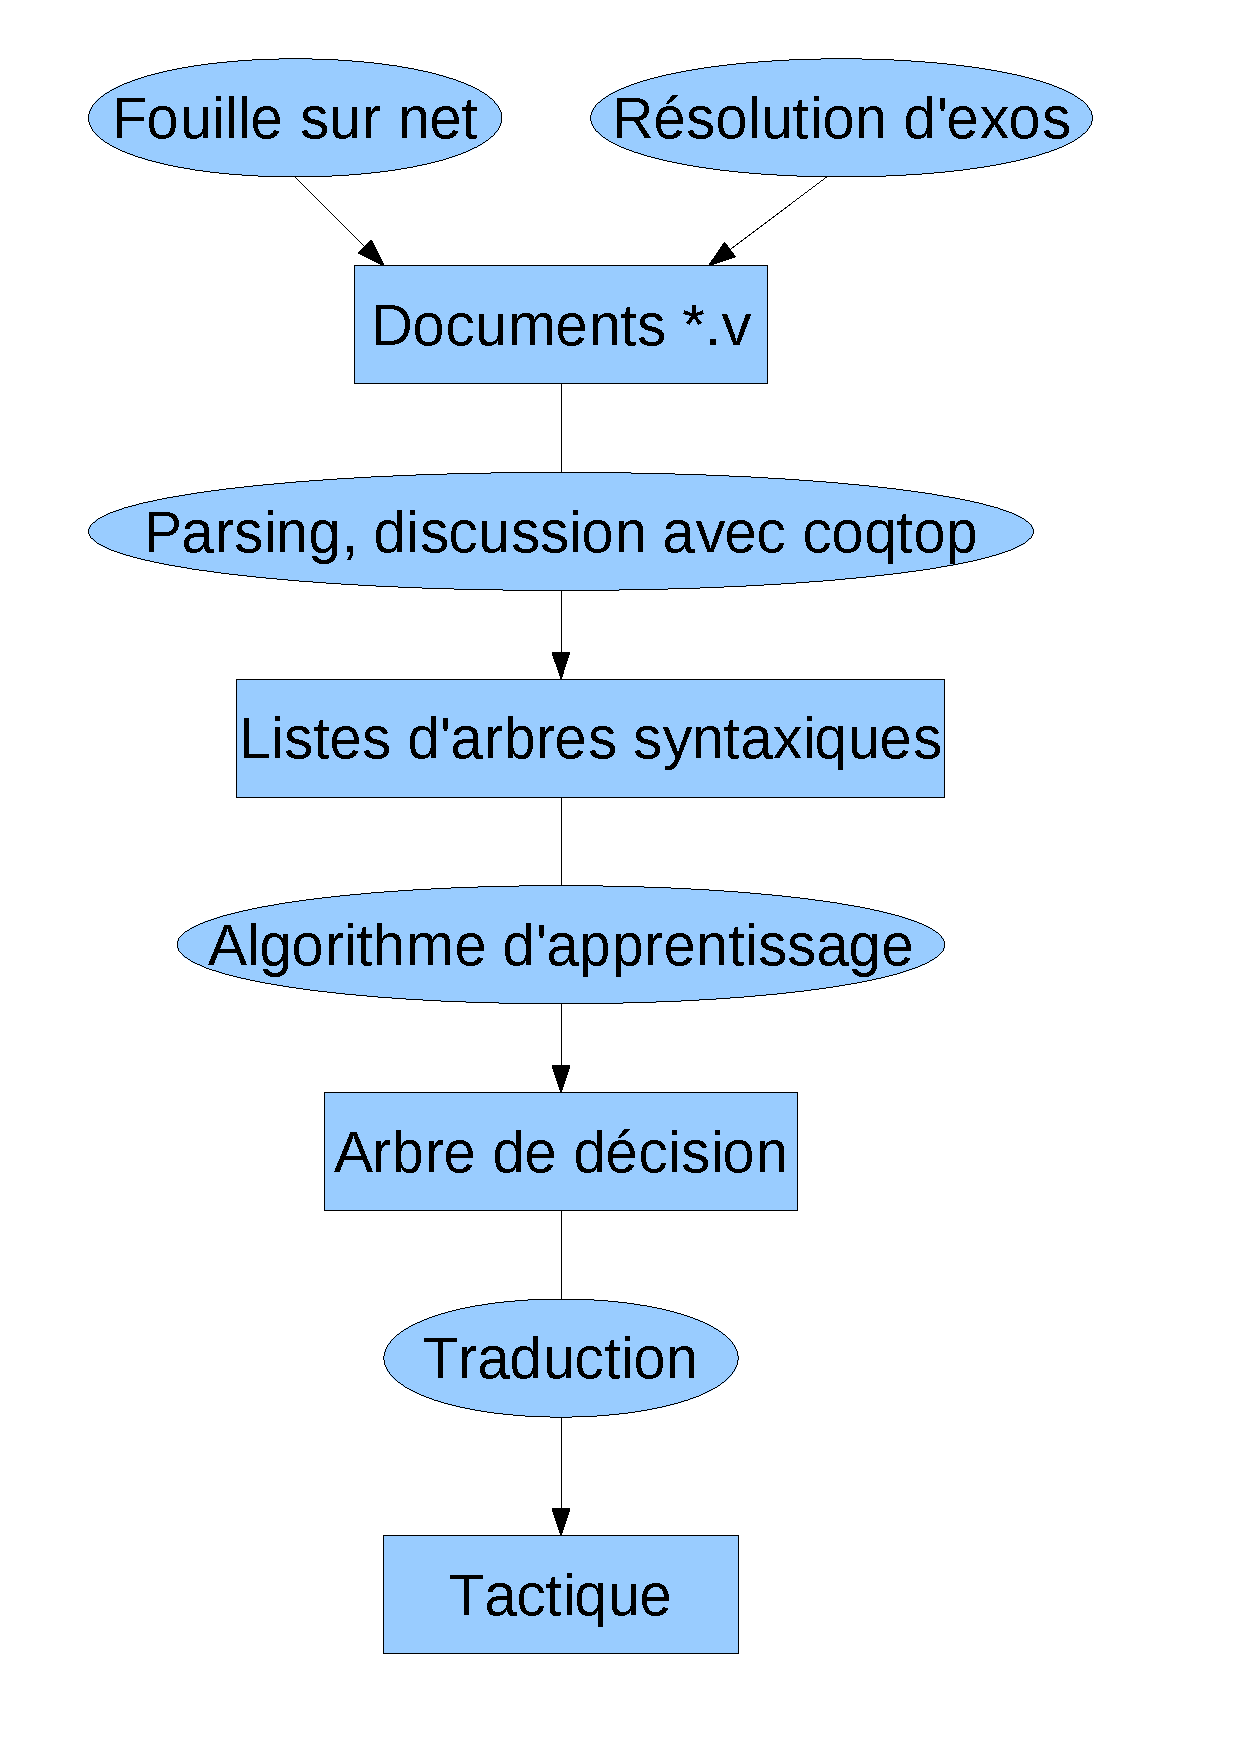
\includegraphics[scale=0.2]{../images/apprentissage/organisation_apprentissage.pdf}
\end{minipage}

\end{frame}

\begin{frame}
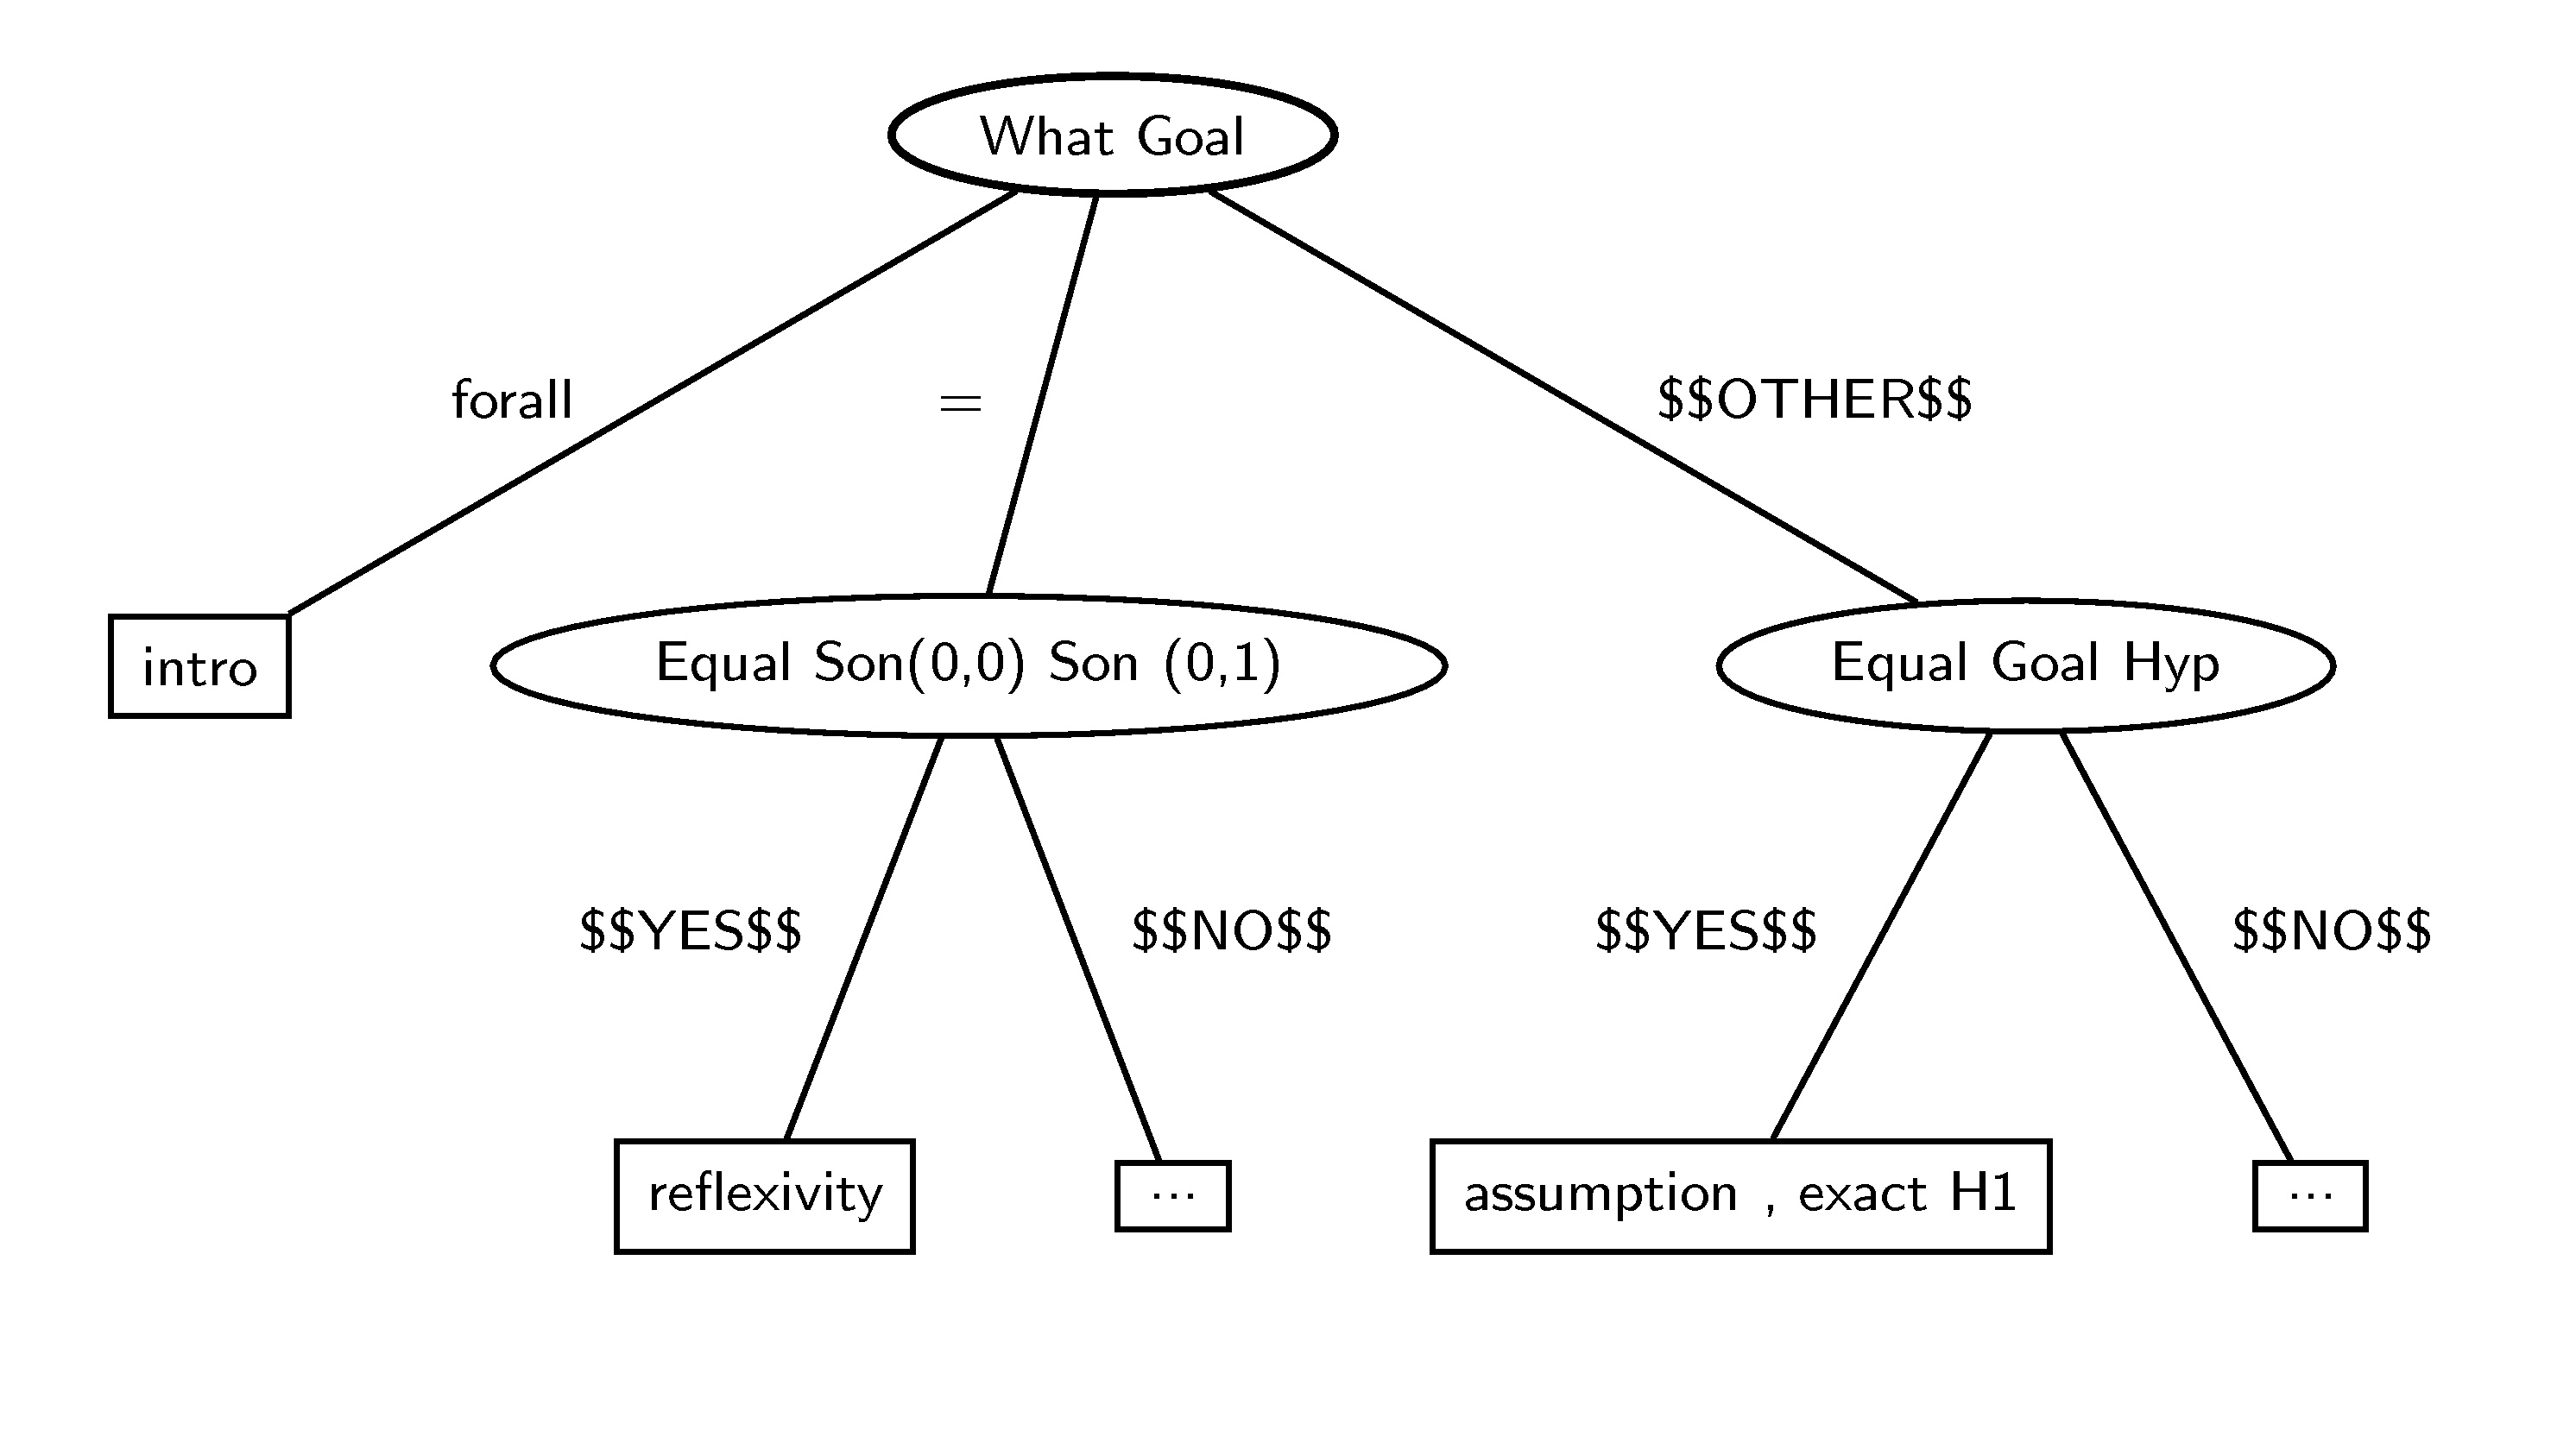
\includegraphics{../images/apprentissage/decision_tree.jpg}
\end{frame}

\begin{frame}

  L'idée
  \begin{itemize}
  \item Réponse sûre au plus vite
  \item On choisit les questions diminuant le plus l'information restante
  \end{itemize}

  Difficultés
  \begin{itemize}
    \item Grand nombre de questions possibles
    \item Multiplicité des réponses à une même question pour un même exemple
    \item Renumérotation des hypothèses
    \item Questions non fixes
  \end{itemize}


\end{frame}


\begin{frame}
\frametitle{Pipeau?}
\begin{itemize}
\item Supposition d'une distribution représentative \\
  $\rightarrow$ Problèmes très classiques, redondant
\item Pas l'arbre le plus petit en théorie \\
  $\rightarrow$ En pratique, ça marche
\item Choix restreint sur les questions\\
  $\rightarrow$ Souvent comme ça qu'on réflechit
\end{itemize}
\end{frame}


\begin{frame}
\frametitle{Résultats}

\begin{itemize}
    \item Le parcours d'arbres et le raffinement des données sont utilisables.
    \item L'algorithme d'apprentissage a été réalisé.
\end{itemize}

\end{frame}
